\documentclass[11pt]{amsart}

\usepackage{amsmath,amssymb,amsthm}
\usepackage{graphicx}
\usepackage[hidelinks]{hyperref}

\newtheorem{theorem}{Theorem}
\newtheorem{corollary}{Corollary}

\newcommand{\Lone}{L_1(\nu)}
\newcommand{\Linfty}{L_\infty(\nu)}
\newcommand{\eps}{\varepsilon}
\newcommand{\N}{\mathbb N}

\title[Canonical interval reduction]{A Canonical Order-Interval Reduction for Question 1.2 of arXiv:2404.05419}
\author{agent\_lane\_15}
\date{June 28, 2026}

\begin{document}
\maketitle

\section*{Source and Target Question}

The source paper is Jose Rodriguez, \emph{Dunford-Pettis type properties in
$L_1$ of a vector measure}, arXiv:2404.05419.  In the introduction Rodriguez
asks the following question.

\begin{quote}
Suppose that $L_1(\nu)$ has the positive Schur property. Does $L_1(\nu)$ have
the Dunford-Pettis property?
\end{quote}

\begin{center}
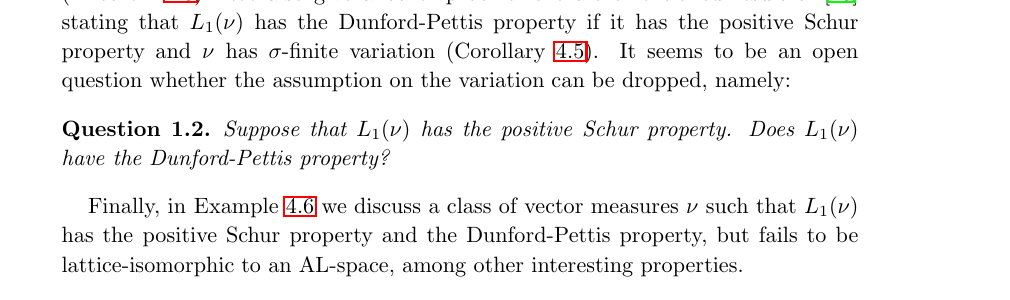
\includegraphics[width=0.92\linewidth]{figures/question_1_2_crop.png}
\end{center}

\section*{Definitions and Source Facts Used}

Let $X$ be a Banach space, let $(\Omega,\Sigma)$ be a measurable space, and let
$\nu\in{\rm ca}(\Sigma,X)$.  Write $E=\Lone$ and let
\[
        j_\nu:\Linfty\longrightarrow \Lone
\]
be the canonical inclusion.  Rodriguez notes in Section 2 that
\[
        K_\nu:=j_\nu(B_{\Linfty})
             =[-\chi_\Omega,\chi_\Omega]
\]
is a weakly compact order interval in $E$.

A bounded subset $K$ of a Banach space $E$ is a Dunford-Pettis set if every
weakly null sequence $(\varphi_n)$ in $E^*$ converges uniformly to zero on $K$,
that is,
\[
        \sup_{x\in K} |\varphi_n(x)|\longrightarrow 0.
\]
We use the standard sequential characterization of the Dunford-Pettis property:
$E$ has the Dunford-Pettis property if and only if
\[
        \varphi_n(x_n)\longrightarrow 0
\]
for all weakly null sequences $(x_n)$ in $E$ and $(\varphi_n)$ in $E^*$.
This is the criterion quoted in Rodriguez before Theorem 4.1.

We also use two preliminary facts recorded by Rodriguez.  First, a Banach
lattice has the positive Schur property if and only if every relatively weakly
compact subset is L-weakly compact.  Second, for subsets of $\Lone$, L-weak
compactness is equivalent to approximate order boundedness: for every
L-weakly compact $F\subset \Lone$ and every $\eps>0$, there is $\rho>0$ such
that
\[
        F\subset j_\nu(\rho B_{\Linfty})+\eps B_{\Lone}.
\]
These are Propositions 2.4 and 2.5 of the source paper.

\section*{Main Reduction}

\begin{theorem}
Let $\nu\in{\rm ca}(\Sigma,X)$ and suppose that $E=\Lone$ has the positive
Schur property.  Then the following are equivalent.
\begin{enumerate}
\item $E$ has the Dunford-Pettis property.
\item $K_\nu=j_\nu(B_{\Linfty})=[-\chi_\Omega,\chi_\Omega]$ is a
      Dunford-Pettis subset of $E$.
\item The adjoint $j_\nu^*:E^*\to\Linfty^*$ is a Dunford-Pettis operator.
\end{enumerate}
\end{theorem}

\begin{proof}
First assume that $E$ has the Dunford-Pettis property.  Since $K_\nu$ is
weakly compact, it is a Dunford-Pettis set.  For completeness, here is the
short sequential argument.  Let $(\varphi_n)$ be weakly null in $E^*$ and
suppose uniform convergence on $K_\nu$ fails.  Passing to a subsequence, choose
$u_n\in K_\nu$ and $\delta>0$ with $|\varphi_n(u_n)|\geq\delta$ for all $n$.
By weak compactness and Eberlein-Smulian, a further subsequence $(u_{n_k})$
converges weakly to some $u\in E$.  Then
\[
        \varphi_{n_k}(u_{n_k})
        =
        \varphi_{n_k}(u_{n_k}-u)+\varphi_{n_k}(u).
\]
The second term tends to zero because $(\varphi_{n_k})$ is weakly null, and
the first tends to zero by the Dunford-Pettis property applied to the weakly
null sequences $(u_{n_k}-u)$ and $(\varphi_{n_k})$.  This contradicts
$|\varphi_{n_k}(u_{n_k})|\geq\delta$.

Conversely, assume that $K_\nu$ is a Dunford-Pettis set.  Let $(f_n)$ be
weakly null in $E$ and let $(\varphi_n)$ be weakly null in $E^*$.  Put
$M=\sup_n\|\varphi_n\|<\infty$.  The set
$F=\{f_n:n\in\N\}$ is relatively weakly compact.  Since $E$ has the positive
Schur property, Rodriguez's Propositions 2.4 and 2.5 imply that for every
$\eps>0$ there is $\rho>0$ such that
\[
        F\subset j_\nu(\rho B_{\Linfty})+\eps B_E.
\]
For each $n$, choose $h_n\in j_\nu(\rho B_{\Linfty})=\rho K_\nu$ with
$\|f_n-h_n\|\leq\eps$.  Since scalar multiples of Dunford-Pettis sets are
Dunford-Pettis sets,
\[
        |\varphi_n(h_n)|\leq
        \sup_{h\in \rho K_\nu}|\varphi_n(h)|
        \longrightarrow 0.
\]
Therefore
\[
        \limsup_n |\varphi_n(f_n)|
        \leq
        \limsup_n |\varphi_n(h_n)| + M\eps
        \leq M\eps.
\]
As $\eps>0$ is arbitrary, $\varphi_n(f_n)\to0$.  The sequential criterion gives
the Dunford-Pettis property of $E$.

Finally, (2) and (3) are the same condition written in dual operator form.  For
every $\varphi\in E^*$,
\[
        \|j_\nu^*\varphi\|
        =
        \sup_{g\in B_{\Linfty}} |\varphi(j_\nu g)|
        =
        \sup_{u\in K_\nu} |\varphi(u)|.
\]
Thus $K_\nu$ is a Dunford-Pettis set exactly when $j_\nu^*$ maps weakly null
sequences in $E^*$ to norm-null sequences in $\Linfty^*$.
\end{proof}

\section*{Conditional Consequence for the Open Question}

\begin{corollary}
A positive answer to Rodriguez's Question 1.2 is equivalent to the following
canonical interval assertion: whenever $\Lone$ has the positive Schur property,
$j_\nu(B_{\Linfty})$ is a Dunford-Pettis subset of $\Lone$.
\end{corollary}

\begin{proof}
If the canonical interval assertion holds, the theorem gives the
Dunford-Pettis property.  Conversely, if Question 1.2 has a positive answer,
then every such $\Lone$ has the Dunford-Pettis property, and the theorem gives
that the canonical interval is a Dunford-Pettis set.
\end{proof}

\section*{Relation to the Sigma-Finite Variation Case}

Rodriguez proves in Corollary 4.5 that the answer is positive when $\nu$ has
$\sigma$-finite variation.  In the language of the reduction above, Proposition
4.4 of the source paper verifies the canonical interval condition in that
case: sequences in $j_\nu(B_{\Linfty})$ are bounded and equi-integrable, so
weakly null functionals in $\Lone^*$ converge to zero on paired sequences from
that interval.

\section*{Limitations and Novelty Check}

This packet is not a full solution of Question 1.2.  It proves an exact
reduction: after assuming the positive Schur property, the full question is
equivalent to proving that one specific weakly compact order interval is a
Dunford-Pettis set.  The remaining dependency is isolated, but not proved here.

Cheap run-index searches for arXiv:2404.05419, the source title, the phrase
``positive Schur property'', and the exact wording of Question 1.2 found no
existing solution packet for this target.  A bounded web search for the exact
question and close variants returned the source paper and adjacent Banach
lattice literature, but no separate resolution of Question 1.2.

\section*{Human Review Recommendation}

The argument is short and should be reviewable directly.  The main points to
check are:
\begin{itemize}
\item the use of Rodriguez's approximate order-boundedness characterization;
\item the standard implication that weak compact subsets of a Dunford-Pettis
      space are Dunford-Pettis sets;
\item the operator wording: the interval condition is equivalent to
      $j_\nu^*$ being Dunford-Pettis, not to $j_\nu$ being Dunford-Pettis.
\end{itemize}

\begin{thebibliography}{9}

\bibitem{Rodriguez2024}
J. Rodriguez,
\emph{Dunford-Pettis type properties in $L_1$ of a vector measure},
arXiv:2404.05419, 2024.

\bibitem{Andrews1979}
K. T. Andrews,
\emph{Dunford-Pettis sets in the space of Bochner integrable functions},
Mathematische Annalen 241 (1979), 35--41.

\bibitem{AliprantisBurkinshaw}
C. D. Aliprantis and O. Burkinshaw,
\emph{Positive Operators},
Springer, 2006.

\bibitem{MeyerNieberg}
P. Meyer-Nieberg,
\emph{Banach Lattices},
Springer, 1991.

\end{thebibliography}

\end{document}
